

%% AP Physics MC Questions Archive
%%----------------------------------------


%% Defintion of Work
%%----------------------------------------
\element{ap}{
\begin{question}{definition-work-q01}
    %Base your answer to the following question on
    The force vs. distance graph below is for an object being pushed along a straight line,
        starting at rest.
    \begin{center}
    \begin{tikzpicture}
        \begin{axis}[
            axis y line=left,
            axis x line=bottom,
            axis line style={->},
            xlabel={distance},
            x unit=\si{\meter},
            xtick={0,2,4,6},
            minor x tick num=1,
            ylabel={force},
            y unit=\si{\newton},
            ytick={0,5,10,15,20},
            minor y tick num=1,
            xmin=0,xmax=6.2,
            ymin=0,ymax=22,
            grid=major,
            width=0.8\columnwidth,
            height=0.5\columnwidth,
        ]
        \addplot[line width=1pt,mark=\empty] plot coordinates {(0,10) (2,0) (3,20) (6,20)};
        \end{axis}
    \end{tikzpicture}
    \end{center}
    After the object has moved a distance of \SI{2.0}{\meter},
        how much work has been done on it?
    \begin{multicols}{3}
    \begin{choices}
        \wrongchoice{\SI{5}{\joule}}
      \correctchoice{\SI{10}{\joule}}
        \wrongchoice{\SI{15}{\joule}}
        \wrongchoice{\SI{20}{\joule}}
        \wrongchoice{\SI{25}{\joule}}
    \end{choices}
    \end{multicols}
\end{question}
}

\newcommand{\apWorkQTwo}{
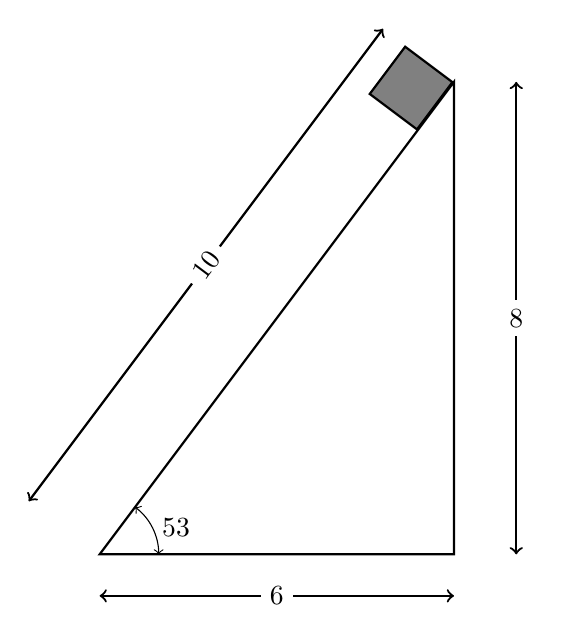
\begin{tikzpicture}[scale=0.75]
    %% Triangle
    \draw[thick] (0,0) -- (6,0) -- (6,8) -- cycle;
    %% Labels
    \draw[<->] (1,0) arc (0:53.13:1) node[pos=0.5,anchor=west] {\ang{53}};
    \draw[<->,thick] (0,-2em) -- (6,-2em) node[pos=0.5,anchor=center,fill=white] {\SI{6}{\meter}};
    \draw[<->,thick] (6cm+3em,0) -- (6cm+3em,8) node[pos=0.5,anchor=center,fill=white] {\SI{8}{\meter}};
    \draw[<->,thick] (143.13:1.5) -- ++(53.13:10) node[pos=0.5,anchor=center,rotate=53.13,fill=white] {\SI{10}{\meter}};
    %% block
    \node[draw,thick,minimum size=0.75cm,fill=white!50!black,rotate=53.13,anchor=south east] (A) at (53.13:10cm) {};
\end{tikzpicture}
}

\element{ap}{
\begin{question}{definition-work-q02}
    Base your answers to the following question on the picture below,
    \begin{center}
        \apWorkQTwo
    \end{center}
        which represents a plane \SI{10}{\meter} in length with a coefficient of kinetic friction of \num{0.2},
        inclined at an angle of \ang{53}.
    A block of weight \SI{30}{\newton} is placed at the top of the plane and allowed to slide down.
    %% Start Question
    The work done on the block by the gravitational force during its \SI{10}{\meter} slide down the plane is most nearly:
    \begin{multicols}{3}
    \begin{choices}
        \wrongchoice{\SI{60}{\joule}}
        \wrongchoice{\SI{180}{\joule}}
        %% NOTE: changed 260 J to 240 J
      \correctchoice{\SI{240}{\joule}}
        \wrongchoice{\SI{300}{\joule}}
        \wrongchoice{\SI{390}{\joule}}
    \end{choices}
    \end{multicols}
\end{question}
}

\element{ap}{
\begin{question}{definition-work-q03}
    Base your answers to the following question on the picture below,
    \begin{center}
        \apWorkQTwo
    \end{center}
        which represents a plane \SI{10}{\meter} in length with a coefficient of kinetic friction of \num{0.2},
        inclined at an angle of \ang{53}.
    A block of weight \SI{30}{\newton} is placed at the top of the plane and allowed to slide down.
    %% Start Question
    The work done on the block by friction during its \SI{10}{\meter} slide down the plane is most nearly:
    \begin{multicols}{3}
    \begin{choices}
        \wrongchoice{\SI{10}{\joule}}
        \wrongchoice{\SI{12}{\joule}}
        \wrongchoice{\SI{18}{\joule}}
        \wrongchoice{\SI{24}{\joule}}
      \correctchoice{\SI{36}{\joule}}
    \end{choices}
    \end{multicols}
\end{question}
}

\element{ap}{
\begin{question}{definition-work-q04}
    Which of the following is not a vector quantity?
    \begin{multicols}{2}
    \begin{choices}
        \wrongchoice{Torque}
        \wrongchoice{Velocity}
      \correctchoice{Work}
        \wrongchoice{Momentum}
        \wrongchoice{Force}
    \end{choices}
    \end{multicols}
\end{question}
}

%\element{ap}{
%\begin{question}{definition-work-q05}
%    A block of mass $M$ is pulled by a constant force $F$ at an angle of \ang{30} relative to the ground for a distance of $L$ meters.
%    \begin{center}
%    \begin{tikzpicture}
%        %% NOTE:
%    \end{tikzpicture}
%    \end{center}
%    What is the net work done?
%    \begin{multicols}{2}
%    \begin{choices}
%        \wrongchoice{$MLF\cos\ang{30}$}
%      \correctchoice{$LF\cos\ang{30}$}
%        \wrongchoice{$L\cos\ang{30}$}
%        \wrongchoice{$\dfrac{F\cos\ang{30}}{ML}$}
%        \wrongchoice{$\dfrac{ML\cos30}{F}$}
%    \end{choices}
%    \end{multicols}
%\end{question}
%}

\element{ap}{
\begin{question}{definition-work-q06}
    A ball of mass \SI{16}{\kilo\gram} on the end of a string is spun at a constant speed of \SI{2.0}{\meter\per\second} in a horizontal circle with a radius of \SI{1}{\meter}.
    What is the work done by the centripetal force during one complete revolution?
    \begin{multicols}{3}
    \begin{choices}
      \correctchoice{\SI{0}{\joule}}
        \wrongchoice{\SI{16}{\joule}}
        \wrongchoice{\SI{32}{\joule}}
        \wrongchoice{\SI{8}{\joule}}
        \wrongchoice{\SI{4}{\joule}}
    \end{choices}
    \end{multicols}
\end{question}
}

\element{ap}{
\begin{question}{definition-work-q07}
    A woman pushes a lawn mower with a force of $F$ at an angle $\theta$ to the ground.
    \begin{center}
    \begin{tikzpicture}
        %% NOTE: tikz or just includegraphic??
        %% NOTE: possible dup from nysed??
    \end{tikzpicture}
    \end{center}
    If $F=\SI{20}{\newton}$ and $\theta=\ang{30}$,
        what is the net work done in moving the lawnmower \SI{5}{\meter}?
    \begin{multicols}{3}
    \begin{choices}
        \wrongchoice{\SI{25}{\joule}}
        \wrongchoice{\SI{50}{\joule}}
      \correctchoice{\SI{86.67}{\joule}}
        \wrongchoice{\SI{14.4}{\joule}}
        \wrongchoice{\SI{35}{\joule}}
    \end{choices}
    \end{multicols}
\end{question}
}

\element{ap}{
\begin{question}{definition-work-q08}
    A vertical force of \SI{500}{\newton} acts on a \SI{12}{\kilo\gram} mass over a horizontal displacement of \SI{2}{\meter}.
    The work done by the force is:
    \begin{multicols}{3}
    \begin{choices}
      \correctchoice{\SI{0}{\joule}}
        \wrongchoice{\SI{24}{\joule}}
        \wrongchoice{\SI{1000}{\joule}}
        \wrongchoice{\SI{6000}{\joule}}
        \wrongchoice{\SI{12000}{\joule}}
    \end{choices}
    \end{multicols}
\end{question}
}

\element{ap}{
\begin{question}{definition-work-q09}
    An object with a mass of \SI{2}{\kilo\gram} is attached to the end of a \SI{3}{\meter} long string and is whirled horizontally in a circle with a constant speed of \SI{5}{\meter\per\second}.
    When the object has traveled half a revolution,
        how much work has been done by the centripetal force?
    \begin{multicols}{3}
    \begin{choices}
      \correctchoice{\SI{0}{\joule}}
        \wrongchoice{$50\pi\,\si{\joule}$}
        \wrongchoice{$100\pi\,\si{\joule}$}
        \wrongchoice{$150\pi\,\si{\joule}$}
        \wrongchoice{$300\pi\,\si{\joule}$}
    \end{choices}
    \end{multicols}
\end{question}
}

\element{ap}{
\begin{question}{definition-work-q10}
    A person lifts a box with a mass of \SI{2.0}{\kilo\gram} from the ground to a shelf \SI{0.5}{\meter} high.
    The work that gravity does on the box is equal to:
    \begin{multicols}{3}
    \begin{choices}
      \correctchoice{\SI{-10}{\joule}}
        \wrongchoice{\SI{-5}{\joule}}
        \wrongchoice{\SI{0}{\joule}}
        \wrongchoice{\SI{5}{\joule}}
        \wrongchoice{\SI{10}{\joule}}
    \end{choices}
    \end{multicols}
\end{question}
}

\element{ap}{
\begin{question}{definition-work-q11}
    If $\mathrm{L}$, $\mathrm{M}$ and $\mathrm{T}$ denote the dimensions of length, mass, and time, respectively, what are the dimensions of energy?
    \begin{multicols}{3}
    \begin{choices}
        \wrongchoice{$\dfrac{\mathrm{M}}{\mathrm{T}^2}$}
        \wrongchoice{$\dfrac{\mathrm{ML}}{\mathrm{T}^2}$}
      \correctchoice{$\dfrac{\mathrm{ML}^2}{\mathrm{T}^2}$}
        \wrongchoice{$\dfrac{\mathrm{M}}{\mathrm{L}^2}$}
        \wrongchoice{$\dfrac{\mathrm{T}^2}{\mathrm{M}}$}
    \end{choices}
    \end{multicols}
\end{question}
}

\element{ap}{
\begin{question}{definition-work-q12}
    How much work is done as a box of weight $W$ is vertically lifted with an acceleration $g$,
        to a height $h$?
    How much work is done against friction?
    \begin{multicols}{3}
    \begin{choices}
      \correctchoice{$Wh$}
        \wrongchoice{$Whg^2$}
        \wrongchoice{$\dfrac{Wh}{g}$}
        \wrongchoice{$\dfrac{2Wh}{g}$}
        \wrongchoice{$2Wh$}
    \end{choices}
    \end{multicols}
\end{question}
}

\element{ap}{
\begin{question}{definition-work-q13}
    A horizontal force of \SI{40}{\newton} is used to push a block along a horizontal surface at a constant speed of \SI{2}{\meter\per\second}.
    How much work is done on the block in \SI{6}{\second}?
    \begin{multicols}{3}
    \begin{choices}
        \wrongchoice{\SI{80}{\joule}}
        \wrongchoice{\SI{120}{\joule}}
        \wrongchoice{\SI{180}{\joule}}
        \wrongchoice{\SI{240}{\joule}}
      \correctchoice{\SI{480}{\joule}}
    \end{choices}
    \end{multicols}
\end{question}
}

%\element{ap}{
%\begin{question}{definition-work-q14}
%    A student pulls a block \SI{3.0}{\meter} along a horizontal surface at constant velocity.
%    The diagram below shows the components of the force exerted on the block by the student.
%    \begin{center}
%    \begin{tikzpicture}
%        %% NOTE:
%    \end{tikzpicture}
%    \end{center}
%    How much work is done against friction?
%    \begin{multicols}{3}
%    \begin{choices}
%        \wrongchoice{\SI{6}{\joule}}
%        \wrongchoice{\SI{18}{\joule}}
%      \correctchoice{\SI{24}{\joule}}
%        \wrongchoice{\SI{30}{\joule}}
%        \wrongchoice{\SI{42}{\joule}}
%    \end{choices}
%    \end{multicols}
%\end{question}
%}

\element{ap}{
\begin{question}{definition-work-q15}
    In order to demonstrate some concepts of physics,
        a physics teacher pushes against a wall with a force of \SI{300}{\newton} for \SI{5}{\second}.
    As you can imagine, the wall remains stationary.
    How much work does the teacher do on the wall in this time period?
    \begin{multicols}{3}
    \begin{choices}
      \correctchoice{\SI{0}{\joule}}
        \wrongchoice{\SI{0.017}{\joule}}
        \wrongchoice{\SI{60}{\joule}}
        \wrongchoice{\SI{750}{\joule}}
        \wrongchoice{\SI{1500}{\joule}}
    \end{choices}
    \end{multicols}
\end{question}
}


\endinput


